\subsection{Positive and Bernstein polynomials}
\label{sec:bernstein}

In physics, it is sometimes necessary to fit data with a function that is
positive everywhere on its domain.  An example of such data is density; it
is a positive quantity and any regression on it should be positive.  In
numerical methods, we often use polynomials as a means of representation, and
hence we want to find polynomials that are positive on some compact domain,
without loss of generality say, $[0,1]$.
It is very difficult to control a polynomial
such that it is positive during the fitting process using a linear constraint
solver. One method used by physicists is to restrict the
fitting process to Bernstein polynomials~\cite{Phillips:2003}. By only using 
positive Bernstein coefficients, Bernstein
polynomials are restricted to be strictly positive.  However,
%based on our interviews with experts,
physicists do not know how ``representative'' are the positive Bernstein
expansions of the space of positive polynomials. In other words, can every
positive polynomial be represented by a corresponding Bernstein polynomial? 
To show these differences, I
select a large number of polynomials and visually compare the spaces in
order to understand the differences.

A Bernstein polynomial of degree \(n\) is a linear combination of
\(n+1\) basis polynomials. 
\[
B_n(x) = \sum_{i=0}^n \beta_i b_{i,n}(x) 
\]
where \(\beta_i\) is a scalar factor and
\(b_{i,n}\) is a Bernstein basis polynomial. These are defined as, 
\[
b_{i,n}(x) = {n \choose i} x^i (1-x)^{n-i}.
\] Each of the
Bernstein basis polynomials is positive in the range \([0,1]\), therefore
if we constrain all \(\beta_i \ge 0\) then the resulting polynomial will
also be positive.

\subsubsection{Sampling method}

The space of a polynomial of degree \(n\) is the range of each of its
coefficients. For example, a 2\textsuperscript{nd} degree polynomial, \(a_0 +
a_1 x + a_2 x^2\), has three coefficients: \(a_0\), \(a_1\), and \(a_2\).
Since we are only concerned with positivity, any polynomials that differ from
each other by a positive factor are equivalent. Thus, the polynomials $0.2x^2 +
0.1x + 2$ and $0.1x^2 + 0.05x + 1$ will be positive in the same range.
Therefore, I constrain the sampling by setting one of the coefficients to $1$
or $-1$ and then sampling the rest between $-1$ and $1$.  I used $10,000$
sample points to get a representative sample.  Since one coefficient is
constrained in turn to either \(-1\) and \(1\) there are \(2n\) possible
polynomials where the remaining \(n\) coefficients range between \([-1,1]\). I
then test to see if each polynomial is positive in the domain \([0,1]\). I also
determine if the equivalent Bernstein polynomial has all \(\beta_i \ge 0\). We
can compute the \(\beta_i\) factors because each coefficient \(a_j\) is a
linear combination of Bernstein coefficients. For our two-dimensional example:
\(a_0 = \beta_0\), \(a_1 = 2(\beta_0-\beta_1)\), and \(a_2=\beta_0 - 2\beta_1 +
\beta_2\). Then, for each polynomial, it is either non-positive, positive
without positive Bernstein coefficients, or positive with positive Bernstein
coefficients. I perform this process to examine polynomials of degree 3, 4, and
5. Constraining a coefficient to $\pm 1$ produces a face of the space of
polynomials. These faces are convex so I can generate a convex hull of these
points and examine them using Hypersliceplorer. Since we are only interested in
how these spaces differ, we examine the difference views.

\begin{figure}
  \centering
  \begin{subfigure}[b]{0.45\linewidth}
    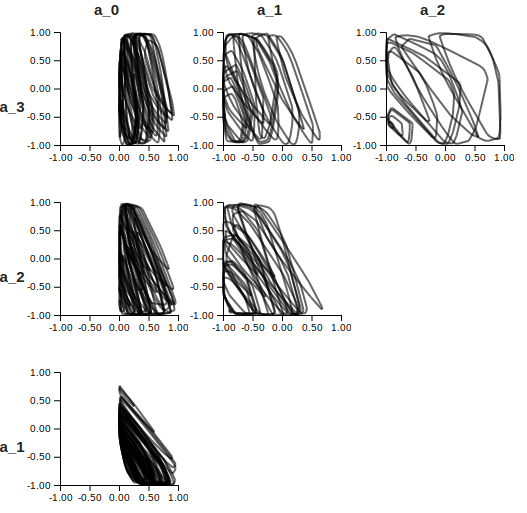
\includegraphics[width=\textwidth]{hsp_d5f1_4-global.png}
    \caption{global view}
    \label{fig:spacediff:global}
  \end{subfigure}
  ~
  \begin{subfigure}[b]{0.45\linewidth}
    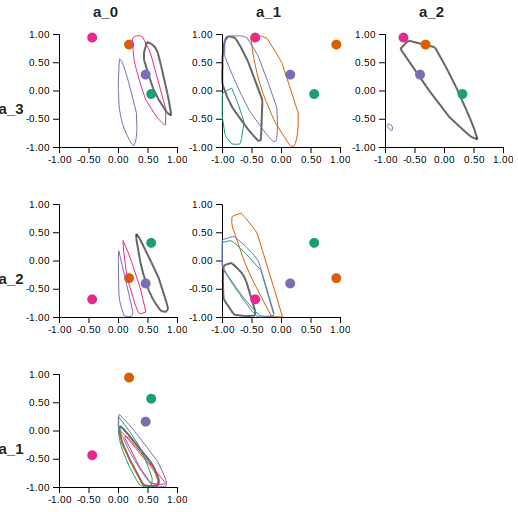
\includegraphics[width=\textwidth]{hsp_d5f1_4-local.png}
    \caption{local view}
    \label{fig:spacediff:local}
  \end{subfigure}
  \caption[Using Hypersliceplorer to examine differences in spaces]{%
    The difference between possible coefficient values for general positive 
    polynomials, $a_0 + a_1 x + a_2 x^2 + a_3 x^3 + x^4$, and polynomials
    that can be represented with positive Bernstein coefficients. From the 
    global view (\subref{fig:spacediff:global}) we can see that the 
    area of the slices is quite large. This means that the 
    difference between spaces is quite large, especially with respect to the
    higher-order coefficients. We can narrow into a particular slice in
    the local view (\subref{fig:spacediff:local}) we can see 
    the orthogonal faces to the slice in the $a_2 \times a_3$ plot.
  }
  \label{fig:spacediff}
\end{figure}

The current assumptions is that, while there is a difference between the set of all positive polynomials and the set of all Bernstein polynomials with positive coefficients,
that difference is small. However, the Hypersliceplorer visualization shows
that this is not the case. \autoref{fig:spacediff:global} 
shows all 4\textsuperscript{th} degree polynomial with the $x^4$ term fixed to
$1$. We can see that for almost an entire range of the $x^2$ and $x^3$
coefficients $a_1, a_2$ there are positive polynomials for which one cannot find a
Bernstein polynomial with positive Bernstein coefficients. Using the local view
(\autoref{fig:spacediff:local}), we can see that this difference is also
large in the other dimensions. Other patterns become apparent, such that $a_0>0$ which could lead to novel hypothesis that can be tested.

\begin{figure*}
  \centering
  \begin{subfigure}[b]{0.3\textwidth}
    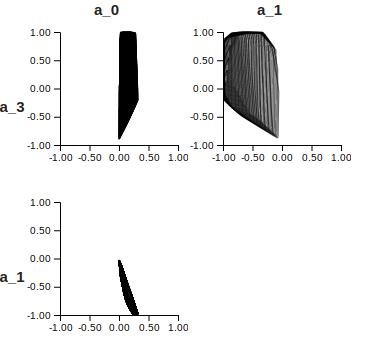
\includegraphics[width=\textwidth]{hsp_d3f1_3.png}
    \caption{degree 3 polynomials}
    \label{fig:dimcmp:3}
  \end{subfigure}
  ~
  \begin{subfigure}[b]{0.3\textwidth}
    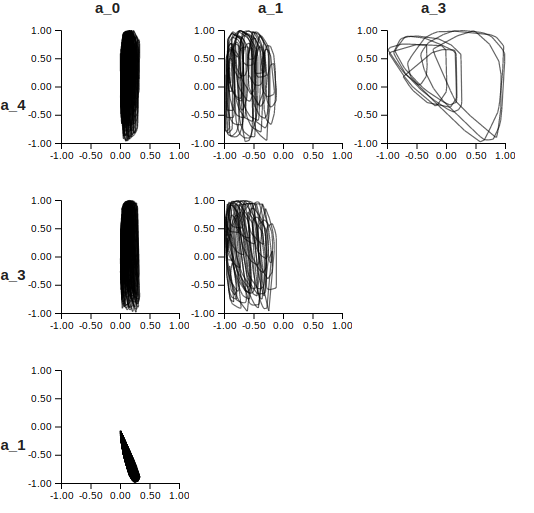
\includegraphics[width=\textwidth]{hsp_d3f1_4.png}
    \caption{degree 4 polynomials}
    \label{fig:dimcmp:4}
  \end{subfigure}
  ~
  \begin{subfigure}[b]{0.3\textwidth}
    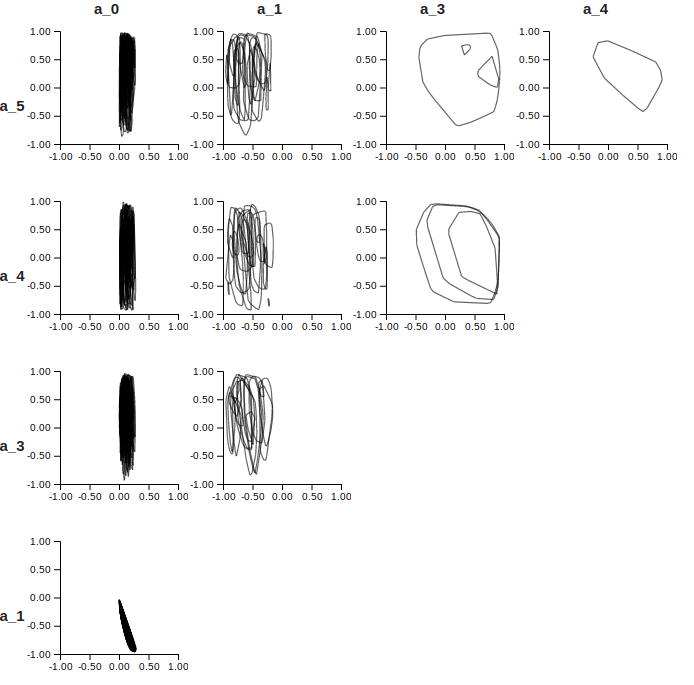
\includegraphics[width=\textwidth]{hsp_d3f1_5.png}
    \caption{degree 5 polynomials}
    \label{fig:dimcmp:5}
  \end{subfigure}
  \caption[Differences in the space of general positive polynomials and Bernstein polynomials with positive Bernstein coefficients.]{%
    Examining differences in the space of general positive polynomials and Bernstein 
    polynomials with positive Bernstein coefficients. In this example the 
    $x^2$ term is set to $1$. We can see that across degrees of polynomials,
    the space differences in the $a_0$ and $a_1$ coefficients is relatively
    consistent. The empty plot in \subref{fig:dimcmp:5} for the $a_3$, $a_4$
    plot is because the focus point sampling did not hit a particular slice.
    The solution is to add additional focus point samples. 
  }
  \label{fig:dimcmp}
\end{figure*}

The global overview also lets us compare across degrees of polynomials.
In \autoref{fig:dimcmp} I show a 3\textsuperscript{rd}, 4\textsuperscript{th},
and 5\textsuperscript{th} degree polynomial with the coefficient of the $x^2$
term set to $1$. Here we can see that the $a_0 \times a_1$ plots all look the same.
In fact, the width across all the panels including $a_0$ are the same. In this
case this means that for these ranges of $a_0$ (the constant term) we will not
be able to find a Bernstein polynomial with positive Bernstein coefficients
no matter the degree of polynomial. 
%\ttwnote{This is because the polynomial coefficients aren't made by that many 
%Bernstein coefficients. Work out the details.}
%\ttwnote{mk: you should be able to use a uniqueness argument.  If you have N+1 points, there is only one polynomial that interpolates it -- a polynomial of degree <= N.  The representation can be monomials, Bernstein, etc.  So, once you "pin" a polynomial (expressed in a monomial expansion), there is but one Bernstein expansion that exists for it; it either has all positive coefficients or not.}


